\documentclass[A4]{article}
\usepackage[T1]{fontenc}
\usepackage{booktabs}
\usepackage{caption}
\usepackage{siunitx}
\usepackage[section]{placeins}
\usepackage{lineno}
\usepackage{graphicx}
\usepackage{url}
\usepackage{authblk}
\usepackage[margin=1in]{geometry}
\newcolumntype{d}{S[input-symbols = ()]}

\renewcommand{\thefigure}{S-\arabic{figure}}
\renewcommand{\thetable}{S-\arabic{table}}
\renewcommand{\theequation}{S-\arabic{equation}}
\renewcommand{\thesection}{S-\arabic{section}}
\renewcommand{\thelinenumber}{S-\arabic{linenumber}}
\renewcommand{\thepage}{Online Resource page \arabic{page}}

\begin{document}

\captionsetup{
    labelfont = bf,
    textfont  = it
  }


\title{Strong spatial and temporal limitations in seed arrival as
  complementary mechanisms for species coexistence in a tropical
  Atlantic coastal forest \\ \ \\
  Published in \emph{Plant Ecology} \\ \ \\
  \textbf{Online Resource}} 

\author[1,2]{Leticia B. Zimback}
\author[2]{Paulo I. Prado}
\author[2]{Marcelo P. Pansonato}
\author[3]{Geraldo A. D. C. Franco}
\author[2,4]{Adriana M. Z. Martini}

\affil[1]{Secretaria do Verde e Meio Ambiente da Prefeitura da Cidade de São Paulo, Brazil}
\affil[2]{Instituto de Biociências, Universidade de São Paulo, Brazil}
\affil[3]{Instituto Florestal do Estado de São Paulo, Brazil}
\affil[4]{Corresponding author, \texttt{amzmartini@usp.br}}


\date{\today}

\maketitle

This appendix provides additional information on the statistical
methods used in the paper and also some supplementary figures and
analyses. All analyses were performed in the R environment
\cite{Rcore}.  R codes and the dataset are available at
\url{https://github.com/piklprado/seedrain}.


\section*{Climate in the study area}

\begin{figure}[!htb]
  \centering
  \includegraphics[width=0.5\textwidth]{../figures/climate_diagram}
  \caption{Climatic diagram from a historical series for the
    Caraguatatuba region, São Paulo State, Brazil. Bars show average
    monthly precipitation from 1943 to 2014 \cite{Santos2019}. Average
    maximum and minimum monthly temperatures are represented by the
    dashed and continuous lines, respectively (data from the last 30
    years, \protect\url{https://www.climatempo.com.br/climatologia/796/caraguatatuba-sp})}
  \label{fig:climate_diag}
\end{figure}

\section*{Spatial and temporal seed limitation}

\subsection*{Descriptive statistics}

\begin{figure}[!htb]
  \centering
  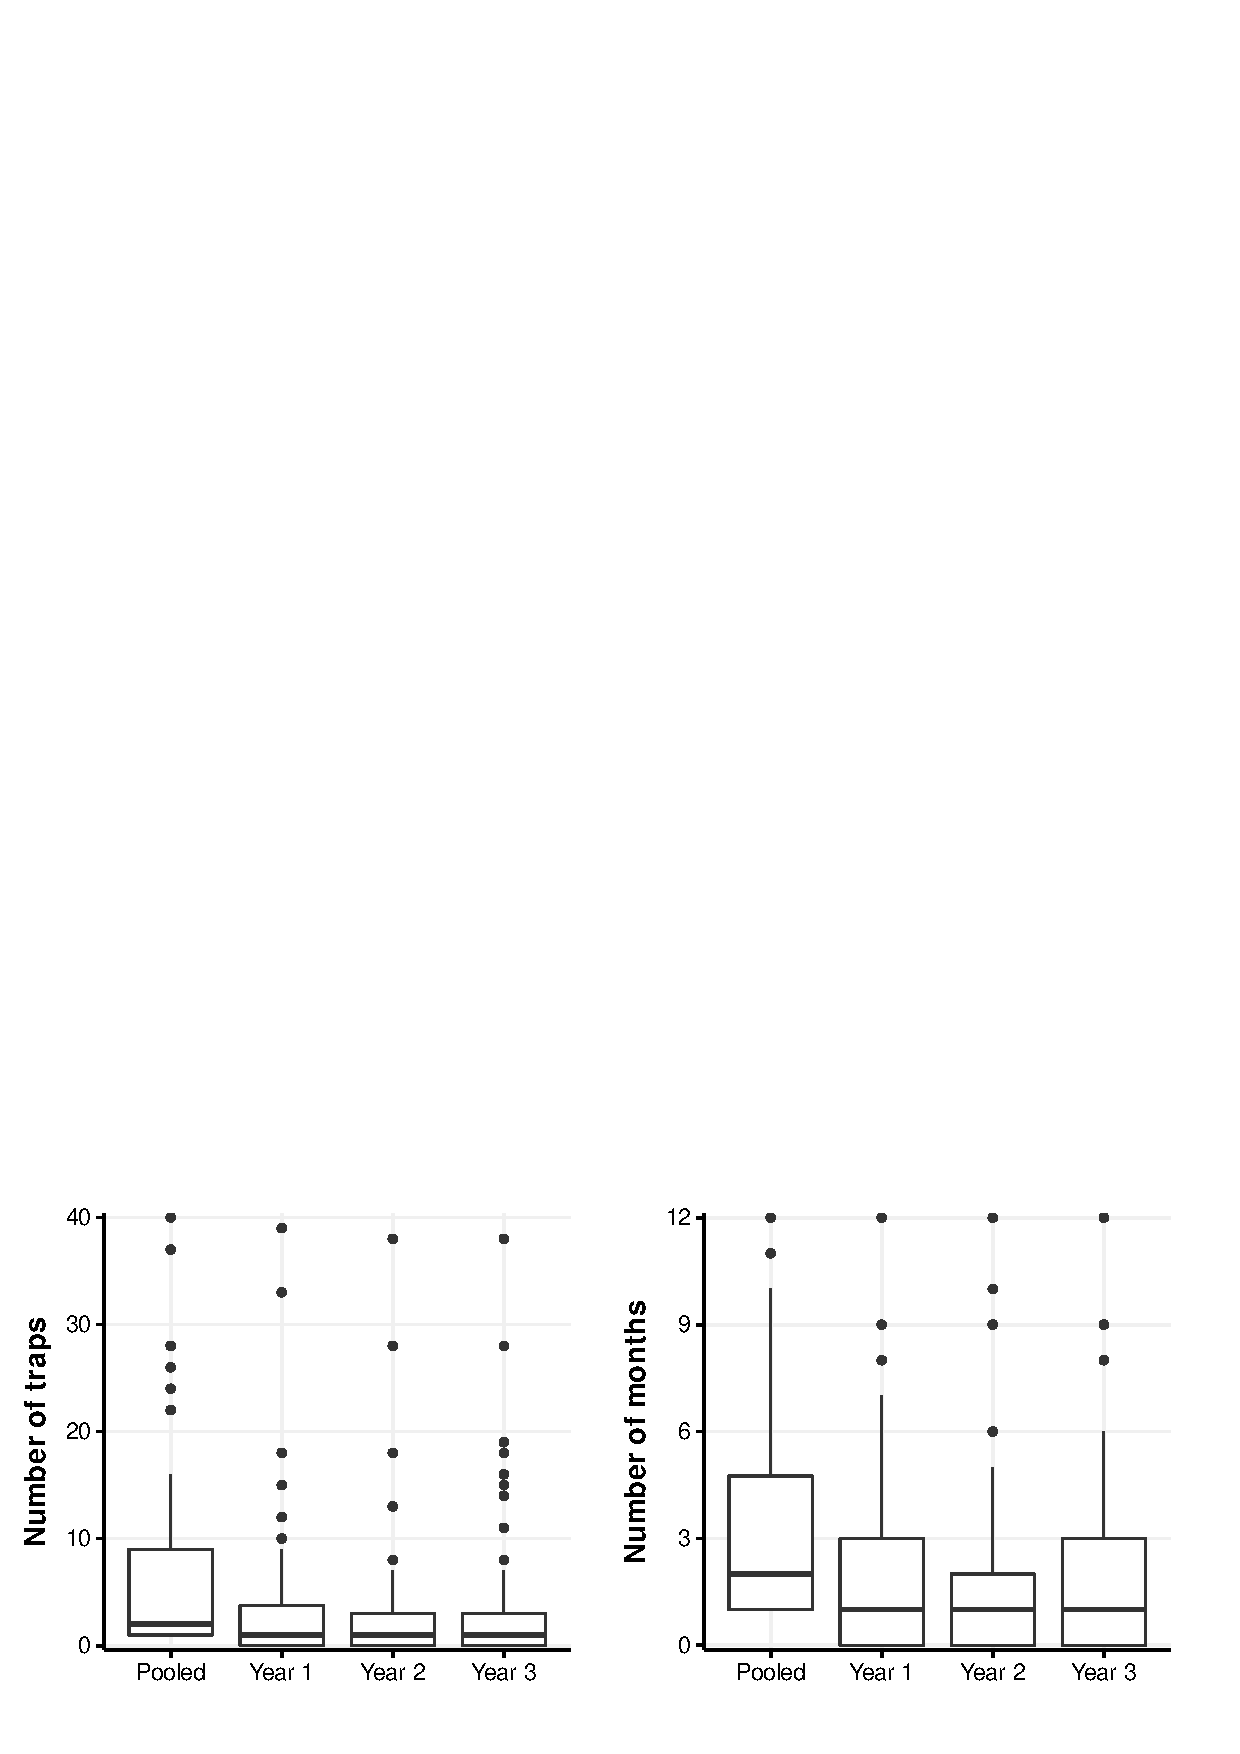
\includegraphics[width=0.65\textwidth]{../figures/frequency_boxplots.pdf}
  \caption{Number of seed traps (left) and months (right) in which the
    seeds of each of the 82 sampled species were recorded for the total
    sampling period (36 months) pooled and for each year separately.}
  \label{fig:freq_seeds}
\end{figure}

\FloatBarrier

\subsection*{Linear models for spatial and temporal seed limitation}
\label{sec:model-select-aver}

In this section we report details of the statistical models used to
describe spatial seed limitation (\emph{SSL}, equation 1 in Methods in
the main paper) and temporal seed limitation (\emph{TSL}, equation
2). We also provide the coefficients of the selected models
($\Delta \mathrm{AICc} \leq 2$), $\mathrm{AICc}$ values for each model and the
coefficients for the average model, obtained from the selected models.


Generalized linear mixed models (glmm) were used to evaluate which
traits were more related to the spatial and/or temporal seed
limitation of the species sampled. As the response variables (SSL and
TSL) are the number of unoccupied traps or months out of a total, a
binomial glmm with the logit link function was used
\cite{bolker2009,dobson2018}. Through the inclusion of random factors,
a mixed model approach allows accounting for hierarchical
relationships and non-independent factors adequately
\cite{bolker2009,Zuur2009book}.  In these models, species identity was
included as a random factor, as there were three values for each
species (i.e., one for each year), and it was expected that temporal
or spatial limitation of the same species was non-independent among
years.

Fixed factors used in the linear models were the following:
\begin{description}
\item[Log seed mass]: logarithm dry seed mass average of each plant
  species. Dry seed mass average were calculated from at least 10
  seeds randomly picked among those collected in the traps (for most
  abundant species, 50 seeds were used);
\item[Adult maximum height]: maximum tree height recorded in the study
  site \cite{pansonato2018}.
\item[Frequency of adults]: proportion of the 40 plots in which a tree
  species was observed in the study site inventory
  \cite{pansonato2018}.
\end{description}


Frequency of adult trees was included to discount the effect of the
spatial distribution of adult individuals on seed limitation. As seed
shadow is strongly concentrated below or nearby adult trees
\cite{flores2013introduced,larios2018}, the presence of a species in a
given seed trap is more probable where an adult individual is present
in the plot. Hence, for spatial seed limitation it would be expected
that a species with a wide spatial distribution of adult individuals
would show low spatial seed limitation. The relationship between
frequency of adult trees and temporal seed limitation is not as
direct. However, species with a broad spatial distribution might be
subjected to more heterogeneous environmental
conditions. Consequently, individuals under distinct conditions (for
example, canopy gaps/closed canopy, flooding/non-flooding) could
promote intraspecific asynchrony among adult individuals of a species
and extend its reproductive period. Hence, a broad spatial
distribution could be related to low temporal seed limitation. Seeds
were also previously classified into two dispersal syndrome
categories, zoochorous and non-zoochorous. However, only four species
(from 31 at total) had non-zoochorous seeds. As this strongly
unbalanced distribution precludes a robust analysis of its effects on
seed limitation, this trait was not used in the analyses.

For each response variable — spatial seed limitation (SSL) or temporal
seed limitation (TSL) — a full glmm model was fit with the glmer
function from the lme4 package \cite{lme4}. In the full model, species
identity was included as a random factor, and all other variables and
their two-way interactions were included as fixed factors. Continuous
fixed factors were standardized by computing z-score values to ease
model convergence \cite{Zuur2009book} and to allow for a direct
comparison of their effects. By using the \emph{dredge} function from
the MuMIn package \cite{MuMIn}, all possible combinations of fixed
factors and two-way interactions were fit and compared. Model
selection was performed using Akaike information criteria (with
correction for small samples) that were calculated with the
\emph{AICc} function from the bbmle package \cite{bbmle}. All models
with $\mathrm{AICc} \leq 2.0$ were considered equally plausible
\cite{Burnham2002}. When multiple models were selected, the average
model was calculated \cite{Burnham2002} using the \emph{model.avg}
function from the MuMIn package \cite{MuMIn} to estimate the effect of
each fixed factor and confidence intervals. Predicted values of the
averaged model were estimated as the average of the fitted values of
each selected model, weighted by their Akaike evidence
weights. $\mathrm{Pseudo-}R^2$ \cite{nakagawa2017} values were
calculated for each selected model using the \emph{r.squaredGLMM}
function from the MuMIn package.

Additionally, generalized linear models (glm) were fitted considering
the total pooled for the 36 months, for both SSL and TSL. For these
analyses, a mixed model was not required because they did not have
repeated values for each species. The procedures of model expansion
using the function \emph{dredge} and model selection were performed in
the same way as described above for the glmm models, but applying
quasi-binomial fitting and quasi-AIC for the model selection were
needed to correct overdispersion of the binomial fits
\cite{Zuur2009book}.

Some species/morphotypes were excluded from the correlation analysis
and from the trait relationships analysis: i) allochthonous seeds
(i.e., seeds of species not recorded as adult trees within the forest
fragment); ii) morphotypes identified only to the genus level, and
with two or more species of this genus among the adults of the forest
site; and iii) species with less than 5 seeds sampled along the three
years, which was stated as a minimum to obtain reliable estimates of
seed limitation.

Tables~\ref{tab:SSL} to \ref{tab:TSL_glm} report the coefficients of
the selected models, $\mathrm{(Q)AICc}$ values for each model and the
coefficients for the average model, obtained from the selected
models. All the fixed-effect variables were standardized as z-values,
to ease convergence of the mixed-effect models, and also to allow
comparison of the coefficients for each effect. We thus refer the
coefficients as ``standardized coefficients''.

Figures~\ref{fig:SSL_glm} and \ref{fig:TSL_glm} show the observed
values of pooled SSL and TSL respectively, and the
predicted values by the fitted generalized linear models.

%\begin{table}

\caption{Mixed-effect models for the spatial seed limation. For each model is shown standarzide coefficients and standard error (brackets).}
\centering
\begin{tabular}[t]{lccccccc}
\toprule
  & 8 & 16 & 7 & 24 & 32 & 6 & Average\\
\midrule
Adult Frequency & \num{-0.410} & \num{-0.303} &  & \num{-0.445} & \num{-0.334} & \num{-0.618} & \num{-0.407}\\
 & (\num{0.226}) & (\num{0.231}) &  & (\num{0.224}) & (\num{0.227}) & (\num{0.218}) & (\num{0.249})\\
Adult height & \num{-0.478} & \num{-0.542} & \num{-0.659} & \num{-0.467} & \num{-0.536} &  & \num{-0.531}\\
 & (\num{0.231}) & (\num{0.227}) & (\num{0.217}) & (\num{0.226}) & (\num{0.221}) &  & (\num{0.238})\\
Log seed mass & \num{1.018} & \num{1.024} & \num{0.975} & \num{1.003} & \num{1.009} & \num{1.029} & \num{1.010}\\
 & (\num{0.205}) & (\num{0.197}) & (\num{0.214}) & (\num{0.201}) & (\num{0.192}) & (\num{0.220}) & (\num{0.208})\\
Frequency:Height &  & \num{-0.320} &  &  & \num{-0.335} &  & \num{-0.326}\\
 &  & (\num{0.234}) &  &  & (\num{0.228}) &  & (\num{0.235})\\
Frequency:Mass &  &  &  & \num{0.257} & \num{0.268} &  & \num{0.262}\\
 &  &  &  & (\num{0.224}) & (\num{0.214}) &  & (\num{0.223})\\
SD (Intercept) & \num{1.022} & \num{0.979} & \num{1.085} & \num{1.002} & \num{0.952} & \num{1.113} & \\
SD (Observations) & \num{1.000} & \num{1.000} & \num{1.000} & \num{1.000} & \num{1.000} & \num{1.000} & \\
\midrule
AIC & \num{489.1} & \num{489.3} & \num{490.2} & \num{489.8} & \num{489.8} & \num{491.0} & \\
\bottomrule
\end{tabular}
\end{table}


\begin{table}
\caption{Mixed-effect models for the spatial seed limation. For each
  model is shown standardized coefficients and standard error
  (brackets). Also shown the estimated standard deviation for the
  random effects (SD), the AICc value for each selected model, and the
  coefficients of the average model.}
\centering
\begin{tabular}[t]{lccccccc}
\toprule
  & 8 & 16 & 7 & 24 & 32 & 6 & Average\\
\midrule
Adult Frequency & \num{-0.410} & \num{-0.303} &  & \num{-0.445} & \num{-0.334} & \num{-0.618} & \num{-0.341}\\
 & (\num{0.226}) & (\num{0.231}) &  & (\num{0.224}) & (\num{0.227}) & (\num{0.218}) & (\num{0.270})\\
Adult height & \num{-0.478} & \num{-0.542} & \num{-0.659} & \num{-0.467} & \num{-0.536} &  & \num{-0.473}\\
 & (\num{0.231}) & (\num{0.227}) & (\num{0.217}) & (\num{0.226}) & (\num{0.221}) &  & (\num{0.277})\\
Log seed mass & \num{1.018} & \num{1.024} & \num{0.975} & \num{1.003} & \num{1.009} & \num{1.029} & \num{1.010}\\
 & (\num{0.205}) & (\num{0.197}) & (\num{0.214}) & (\num{0.201}) & (\num{0.192}) & (\num{0.220}) & (\num{0.205})\\
Frequency:Height &  & \num{-0.320} &  &  & \num{-0.335} &  & \num{-0.106}\\
 &  & (\num{0.234}) &  &  & (\num{0.228}) &  & (\num{0.202})\\
Frequency:Mass &  &  &  & \num{0.257} & \num{0.268} &  & \num{0.074}\\
 &  &  &  & (\num{0.224}) & (\num{0.214}) &  & (\num{0.166})\\
SD (Intercept) & \num{1.022} & \num{0.979} & \num{1.085} & \num{1.002} & \num{0.952} & \num{1.113} & \\
SD (Observations) & \num{1.000} & \num{1.000} & \num{1.000} & \num{1.000} & \num{1.000} & \num{1.000} & \\
\midrule
AICc & \num{489.753} & \num{490.276} & \num{490.645} & \num{490.769} & \num{491.099} & \num{491.440} & \\
\bottomrule
\end{tabular}
\label{tab:SSL}
\end{table}


%\begin{table}

\caption{Fixed effects models for the spatial seed limitation pooled over years (see text for details). For each model is shown standardized coefficients and standard error (brackets). Also shown  the QAICc value for each selected model, and the coefficients of the average model.}
\centering
\begin{tabular}[t]{lccccc}
\toprule
  & 8 & 16 & 7 & 6 & Average\\
\midrule
Adult Frequency & \num{-0.363} & \num{-0.164} &  & \num{-0.538} & \num{-0.257}\\
 & (\num{0.203}) & (\num{0.241}) &  & (\num{0.198}) & (\num{0.269})\\
Adult height & \num{-0.432} & \num{-0.528} & \num{-0.597} &  & \num{-0.413}\\
 & (\num{0.227}) & (\num{0.238}) & (\num{0.210}) &  & (\num{0.293})\\
Log seed mass & \num{0.836} & \num{0.851} & \num{0.771} & \num{0.849} & \num{0.826}\\
 & (\num{0.206}) & (\num{0.198}) & (\num{0.199}) & (\num{0.224}) & (\num{0.208})\\
Frequency:Height &  & \num{-0.395} &  &  & \num{-0.100}\\
 &  & (\num{0.237}) &  &  & (\num{0.209})\\
\midrule
QAICc & \num{56.540} & \num{56.920} & \num{56.965} & \num{57.439} & \\
\bottomrule
\end{tabular}
\end{table}


\begin{table}
\caption{Fixed effects models for the spatial seed limitation pooled
  over years (see text for details). For each model is shown
  standardized coefficients and standard error (brackets). Also shown
  the QAICc value for each selected model, and the coefficients of the
  average model.}
\centering
\begin{tabular}[t]{lccccc}
\toprule
  & 8 & 16 & 7 & 6 & Average\\
\midrule
Adult Frequency & \num{-0.363} & \num{-0.164} &  & \num{-0.538} & \num{-0.257}\\
 & (\num{0.203}) & (\num{0.241}) &  & (\num{0.198}) & (\num{0.269})\\
Adult height & \num{-0.432} & \num{-0.528} & \num{-0.597} &  & \num{-0.413}\\
 & (\num{0.227}) & (\num{0.238}) & (\num{0.210}) &  & (\num{0.293})\\
Log seed mass & \num{0.836} & \num{0.851} & \num{0.771} & \num{0.849} & \num{0.826}\\
 & (\num{0.206}) & (\num{0.198}) & (\num{0.199}) & (\num{0.224}) & (\num{0.208})\\
Frequency:Height &  & \num{-0.395} &  &  & \num{-0.100}\\
 &  & (\num{0.237}) &  &  & (\num{0.209})\\
\midrule
QAICc & \num{56.540} & \num{56.920} & \num{56.965} & \num{57.439} & \\
\bottomrule
\end{tabular}
\label{tab:SSL_glm}
\end{table}


\begin{figure}
  \centering
  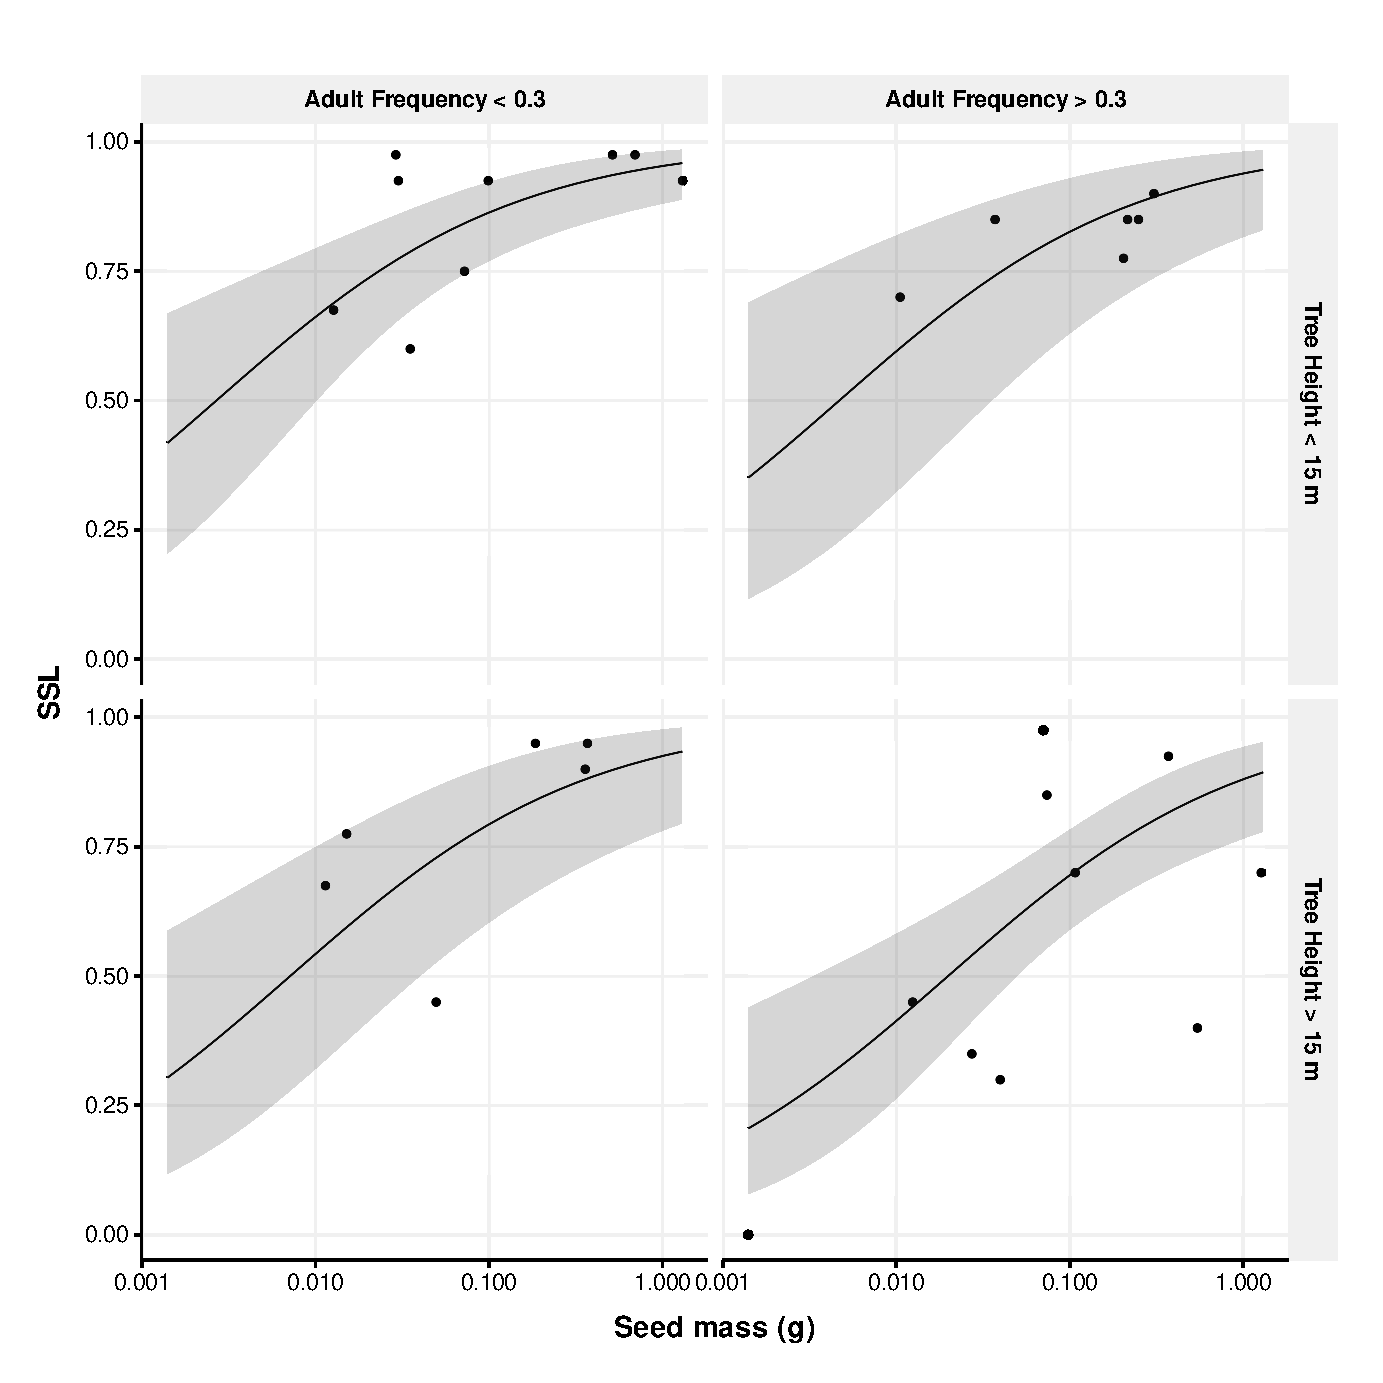
\includegraphics[width=0.5\textwidth]{../figures/SSL_all_pred_prob_glm}
  \caption{Relationship among spatial seed limitation pooled over
    years (SSL), seed mass, tree height, and frequency of adults, as
    predicted by the glm average model (Table~\ref{tab:TSL_glm}). For species with
    frequency lower than median value (0.3) the relationship is showed
    in graphs in the left column, and for those with greater
    frequency, in the right column. For species with tree height lower
    than median value (15 m) the relationship is showed in upper
    graphs, and for those with greater height in bottom
    graphs. Regression lines are predicted values by the average model
    using the midpoint of the height and frequency class in each
    panel. Gray shadows are 95\% prediction interval of the average
    model. Points are observed values of SSL (pooled over the 3 years)
    and seed mass for each species. Note the log scale for seed mass.}
  \label{fig:SSL_glm}
\end{figure}


%\begin{table}
\label{tab:SSL_glm}
\caption{Mixed-effect models for the temporal seed limation. For each model is shown standardized coefficients and standard error (brackets). Also shown the estimated standard deviation for the random effects (SD), the AICc value for each selected model, and the coefficients of the average model.}
\centering
\begin{tabular}[t]{lccccc}
\toprule
  & 7 & 6 & 5 & 8 & Average\\
\midrule
Adult Frequency &  & \num{-0.295} &  & \num{-0.174} & \num{-0.097}\\
 &  & (\num{0.195}) &  & (\num{0.211}) & (\num{0.179})\\
Adult height & \num{-0.355} &  &  & \num{-0.278} & \num{-0.180}\\
 & (\num{0.194}) &  &  & (\num{0.213}) & (\num{0.223})\\
Log seed mass & \num{0.971} & \num{1.000} & \num{0.963} & \num{0.992} & \num{0.979}\\
 & (\num{0.197}) & (\num{0.201}) & (\num{0.206}) & (\num{0.197}) & (\num{0.200})\\
SD (Intercept) & \num{0.919} & \num{0.936} & \num{0.981} & \num{0.905} & \\
SD (Observations) & \num{1.000} & \num{1.000} & \num{1.000} & \num{1.000} & \\
\midrule
AICc & \num{356.252} & \num{357.240} & \num{357.249} & \num{357.819} & \\
\bottomrule
\end{tabular}
\end{table}

\begin{table}
\caption{Mixed-effect models for the temporal seed limation. For each
  model is shown standardized coefficients and standard error
  (brackets). Also shown the estimated standard deviation for the
  random effects (SD), the AICc value for each selected model, and the
  coefficients of the average model.}
\centering
\begin{tabular}[t]{lccccc}
\toprule
  & 7 & 6 & 5 & 8 & Average\\
\midrule
Adult Frequency &  & \num{-0.295} &  & \num{-0.174} & \num{-0.097}\\
 &  & (\num{0.195}) &  & (\num{0.211}) & (\num{0.179})\\
Adult height & \num{-0.355} &  &  & \num{-0.278} & \num{-0.180}\\
 & (\num{0.194}) &  &  & (\num{0.213}) & (\num{0.223})\\
Log seed mass & \num{0.971} & \num{1.000} & \num{0.963} & \num{0.992} & \num{0.979}\\
 & (\num{0.197}) & (\num{0.201}) & (\num{0.206}) & (\num{0.197}) & (\num{0.200})\\
SD (Intercept) & \num{0.919} & \num{0.936} & \num{0.981} & \num{0.905} & \\
SD (Observations) & \num{1.000} & \num{1.000} & \num{1.000} & \num{1.000} & \\
\midrule
AICc & \num{356.252} & \num{357.240} & \num{357.249} & \num{357.819} & \\
\bottomrule
\end{tabular}
\label{tab:SSL_glm}
\end{table}


%\begin{table}

\caption{Fixed effects models for the temporal seed limitation pooled over years (see text for details). For each model is shown standardized coefficients and standard error (brackets). Also shown  the QAICc value for each selected model, and the coefficients of the average model.}
\centering
\begin{tabular}[t]{lcccc}
\toprule
  & 5 & 7 & 6 & Average\\
\midrule
Adult Frequency &  &  & \num{-0.198} & \num{-0.045}\\
 &  &  & (\num{0.182}) & (\num{0.120})\\
Adult height &  & \num{-0.224} &  & \num{-0.059}\\
 &  & (\num{0.185}) &  & (\num{0.137})\\
Log seed mass & \num{0.628} & \num{0.639} & \num{0.661} & \num{0.638}\\
 & (\num{0.193}) & (\num{0.194}) & (\num{0.198}) & (\num{0.194})\\
\midrule
QAICc & \num{62.212} & \num{63.548} & \num{63.812} & \\
\bottomrule
\end{tabular}
\end{table}

\begin{table}
\caption{Fixed effects models for the temporal seed limitation pooled
  over years (see text for details). For each model is shown
  standardized coefficients and standard error (brackets). Also shown
  the QAICc value for each selected model, and the coefficients of the
  average model.}
\centering
\begin{tabular}[t]{lcccc}
\toprule
  & 5 & 7 & 6 & Average\\
\midrule
Adult Frequency &  &  & \num{-0.198} & \num{-0.045}\\
 &  &  & (\num{0.182}) & (\num{0.120})\\
Adult height &  & \num{-0.224} &  & \num{-0.059}\\
 &  & (\num{0.185}) &  & (\num{0.137})\\
Log seed mass & \num{0.628} & \num{0.639} & \num{0.661} & \num{0.638}\\
 & (\num{0.193}) & (\num{0.194}) & (\num{0.198}) & (\num{0.194})\\
\midrule
QAICc & \num{62.212} & \num{63.548} & \num{63.812} & \\
\bottomrule
\end{tabular}
\label{tab:TSL_glm}
\end{table}


\begin{figure}[h!]
  \centering
  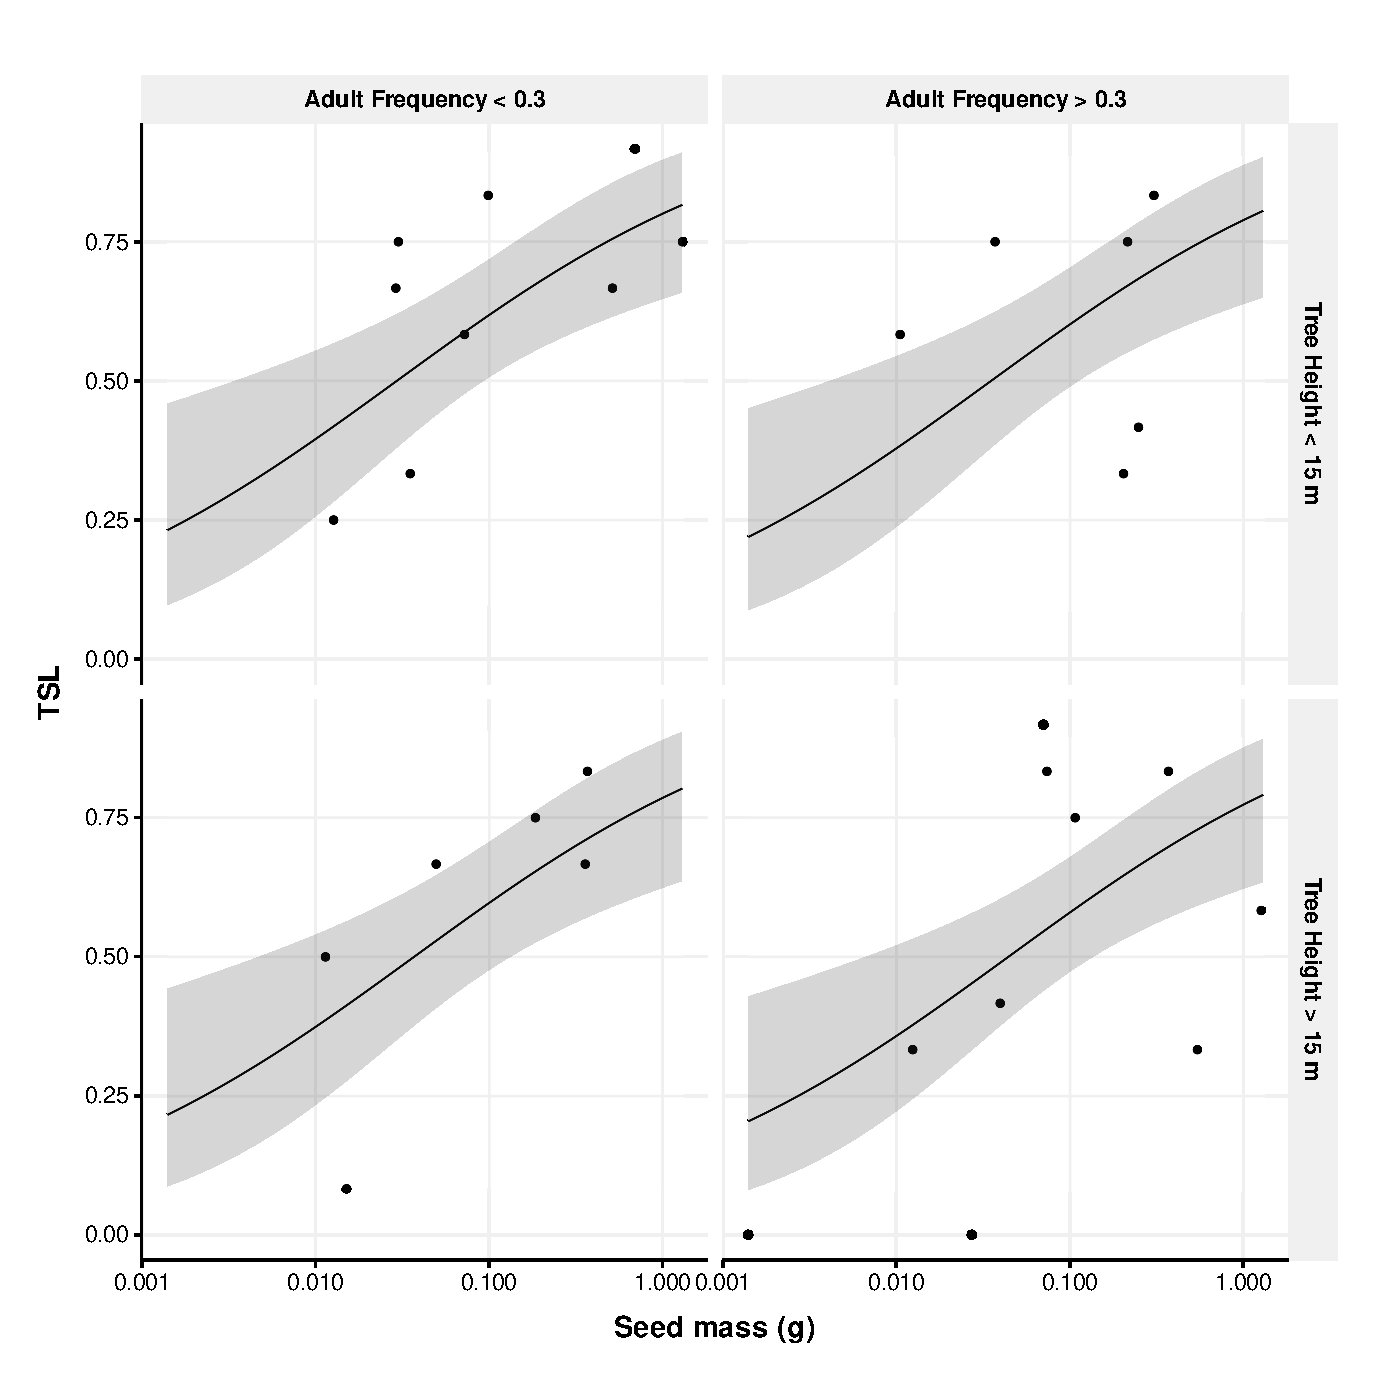
\includegraphics[width=0.5\textwidth]{../figures/TSL_all_pred_prob_glm}
  \caption{Relationship among temporal seed limitation pooled over
    years (TSL), seed mass, tree height, and frequency of adults, as
    predicted by the glm average model (Table~\ref{tab:SSL_glm}). For
    species with frequency lower than median value (0.3) the
    relationship is showed in graphs in the left column, and for those
    with greater frequency, in the right column. For species with tree
    height lower than median value (15 m) the relationship is showed
    in upper graphs, and for those with greater height in bottom
    graphs. Regression lines are predicted values by the average model
    using the midpoint of the height and frequency class in each
    panel. Gray shadows are 95\% prediction interval of the average
    model. Points are observed values of SSL (pooled over the 3 years)
    and seed mass for each species. Note the log scale for seed mass.}
  \label{fig:TSL_glm}
\end{figure}

\FloatBarrier
\section*{Circular statistics of temporal distribution of seeds}
\label{sec:circ-stat-temp}

The mean number of seed species in each month for the three years was
used to calculate a mean distribution vector (r), represented by the
red line in Fig.~\ref{fig:circular}. Small vectors, like the one
seen in Fig.~\ref{fig:circular}, indicate low temporal synchrony and
high uniformity among the months. The calculated value of the mean
distribution vectors was $r=0.0475$, and the Rayleigh Test of
Uniformity (Z) returned a p-value of $p=0.709$, and thus the null
hypothesis of uniform distribution over months can not be
rejected. This figure, the \emph{r} calculation, and the Rayleigh test
were performed with the circular R package \cite{circular}.

\begin{figure}[h!]
  \centering
  \includegraphics[width=0.5\textwidth]{../figures/circular_distribution}
  \caption{Circular distribution of the mean number of seed species in
    each month. The lenght of each sector (month) is the average of
    the number of seed species recorded each month for the tree
    years. Maximum lenght is 16,67 for July. }
  \label{fig:circular}
\end{figure}

\FloatBarrier

\bibliographystyle{acm}
\bibliography{suppl}


\end{document}
